\begin{vbframe}{Linear SVM -- method summary}

% \maketag{SUPERVISED} 
\maketag{CLASSIFICATION} \maketag[50]{REGRESSION} \maketag{PARAMETRIC} 
\maketag{WHITE-BOX} 
\medskip


% \begin{itemize}
%   \item Find linear decision boundary (\textbf{separating hyperplane}) that 
%   best discriminates classes
%   %\begin{itemize}
%     %\item \textbf{Hard-margin} SVM: maximize distance (\textbf{margin} $\gamma$ > 0) to closest points (\textbf{support vectors, SVs}) on each side of decision boundary
%     %\item \textbf{Soft-margin} SVM: relax separation to allow for margin violations $\Rightarrow$ maximize margin while minimizing violations
%   %\end{itemize}
% \end{itemize}

\begin{columns}[T]
\begin{column}{0.7\linewidth}
    
\highlight{General idea (Soft-margin SVM)}
\begin{itemize}
\item Find linear decision boundary (\textbf{separating hyperplane}) that 
\begin{itemize}
    \item maximizes distance (\textbf{margin} $\gamma$) to closest points (\textbf{support vectors, SVs}) on each side of decision boundary
    \item while minimizing margin violations (\textbf{points between dashed margin lines})
\end{itemize}
  \item 3 types of training points
  \begin{itemize}
    \item \textbf{non-SVs} with no impact on decision boundary
    \item \textbf{margin violators} with impact on decision boundary
    \item \textbf{SVs} located exactly on margin borders (affect decision boundary)
  \end{itemize}
  %\item \textbf{Interpretable} weighted sum of scalar product with positive coefficients for support vectors
  %\item Extension to \textbf{regression} is possible but requires modifications 
  %\\ $\Rightarrow$ here: only classification case
\end{itemize}
\end{column}
\begin{column}{0.3\linewidth}
    
  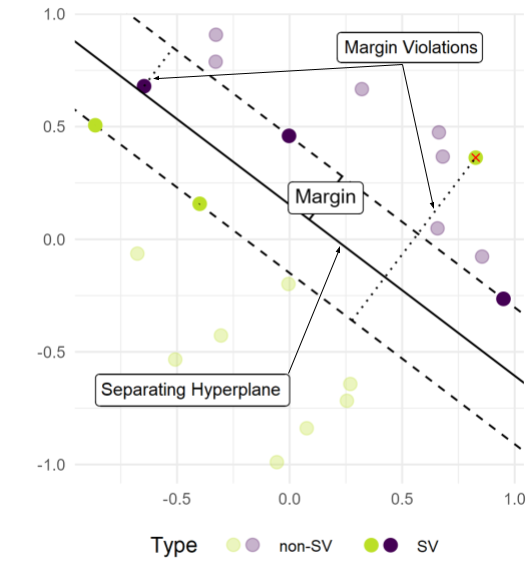
\includegraphics[width=\linewidth]{figure/svm_wording.png} \\
  \tiny{Soft-margin SVM with margin violations}
\end{column}
\end{columns}


\medskip

\highlight{Hypothesis space}\\
%\textcolor{blue}{
$
\Hspace = \left\{\fx ~:~\fx = \thetab^\top \xv + \theta_0 \right\} $ with $   \thetab = \sumin \alpha_i \yi \xi $ ($\alpha_i$ are Lagrange multipliers)

$\Rightarrow$ \textbf{Note:} Non-SVs have $\alpha_i = 0$ as they do not affect the hyperplane

$\Rightarrow \Hspace = \left \{\fx ~:~ \fx = \sumin \alpha_i \yi \langle \xi, \xv \rangle  + \theta_0 ~|~ \alpha_i \geq 0, \forall i \right \}$
%}


\framebreak

% \medskip
% \footnotesize
% \begin{minipage}{0.6\textwidth}
%   \centering
%   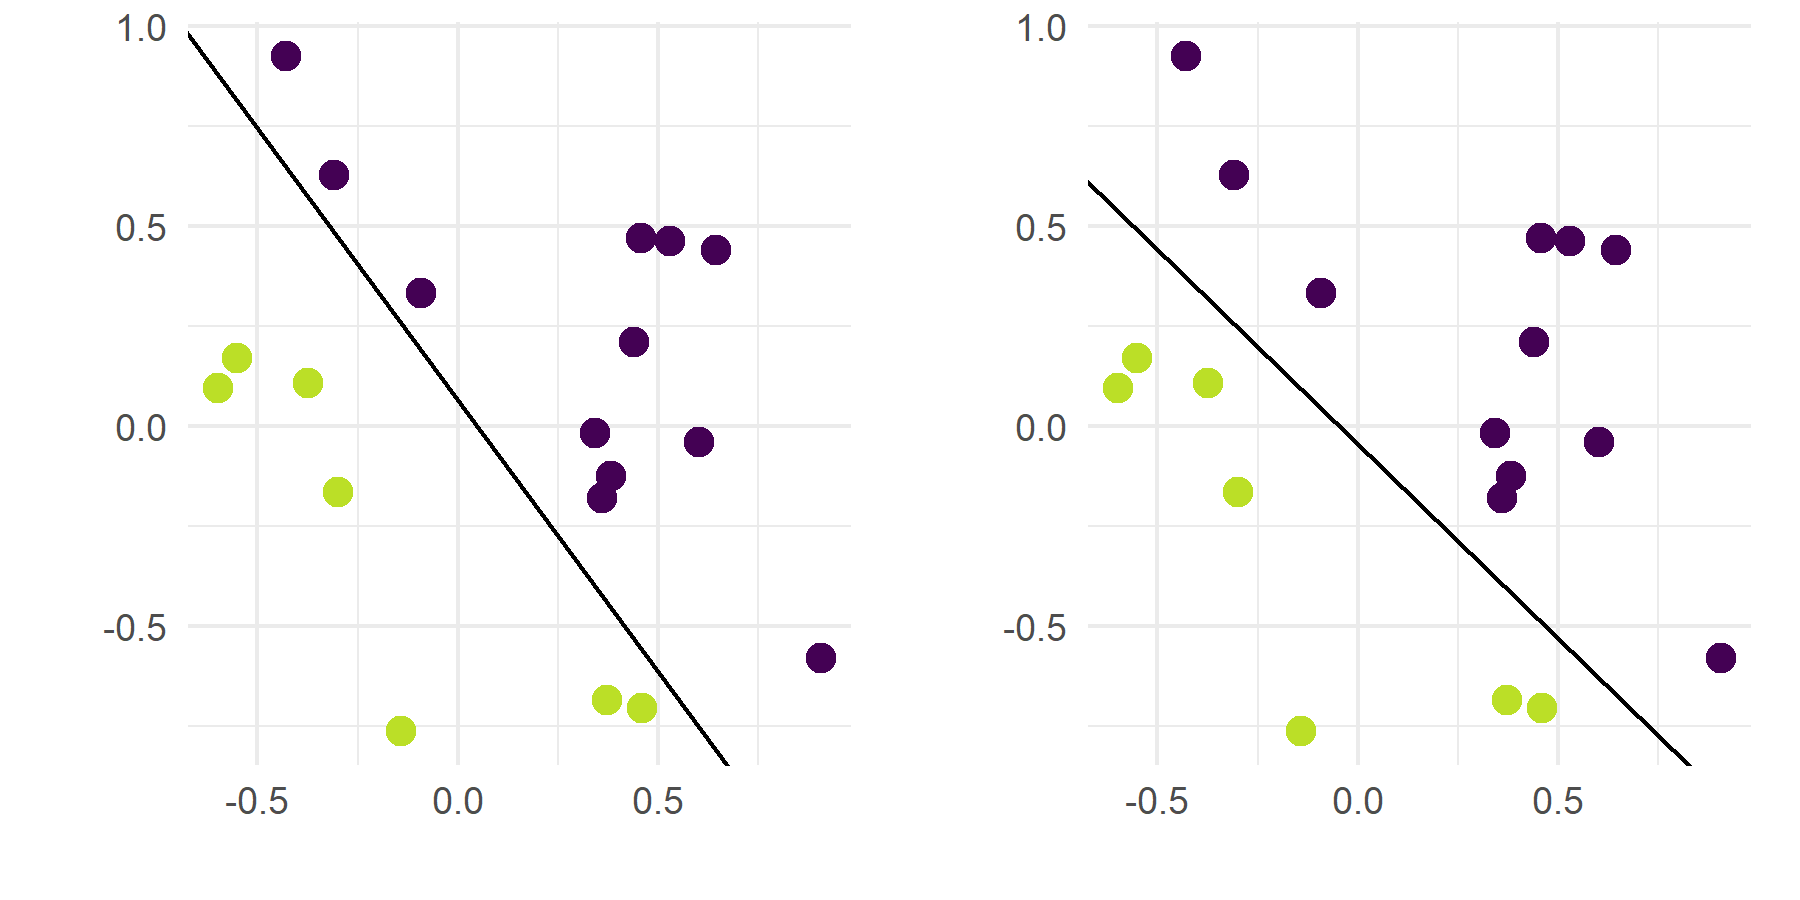
\includegraphics[width=0.9\textwidth]{
%   ../slides/linear-svm/figure/linear_classif_1.png}  \\
%   \tiny{Hard-margin SVM: margin is maximized by boundary on the right}
% \end{minipage}
% \hfill
% \begin{minipage}{0.3\textwidth}
%   \centering
%     %https://docs.google.com/presentation/d/1g7q1hbTNmQeuRWQIM8SF9l6iKWmJyuhyhm3s9QjA0jM/edit?usp=sharing
%   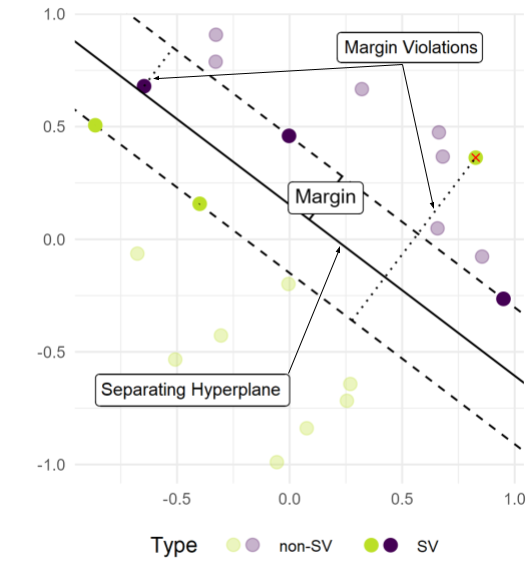
\includegraphics[width=1.1\textwidth]{figure/svm_wording.png} \\
%   \tiny{Soft-margin SVM with margin violations}
% \end{minipage}

\medskip

\begin{columns}[T, totalwidth = \textwidth]
\begin{column}{0.59\textwidth}
    
\highlight{Empirical risk} ~~ Soft-margin SVM as \textbf{L2-regularized ERM}: 
     \centerline{$\frac{1}{2} \|\thetab\|_2^2 + C \sumin \Lxyi$}
     \vspace{-\topsep}
  \begin{itemize}
  \setlength{\parskip}{0pt} 
  \setlength{\itemsep}{0pt plus 1pt}
    \item $\|\thetab\| = 1 / \gamma$ ($\hat{=}$ maximizing margin) \\
    \item $C > 0$: penalization for margin violations
    \item Loss aims at minimizing margin violations\\
    $\rightarrow$ Classif. (\textbf{hinge} loss): $\Lyf = \max(1-yf, 0)$ \\
    %\phantom{$\rightarrow$}$\Rightarrow$ other loss functions applicable (e.g., \textbf{Huber} loss)\\
    $\rightarrow$ Regr. (\textbf{$\eps$-insensitive} loss):   $\Lyf = \max(|y-f| - \eps, 0)$ 
  \end{itemize}
\vspace{-\topsep}
\end{column}
\begin{column}{0.4\textwidth}
  \centering
  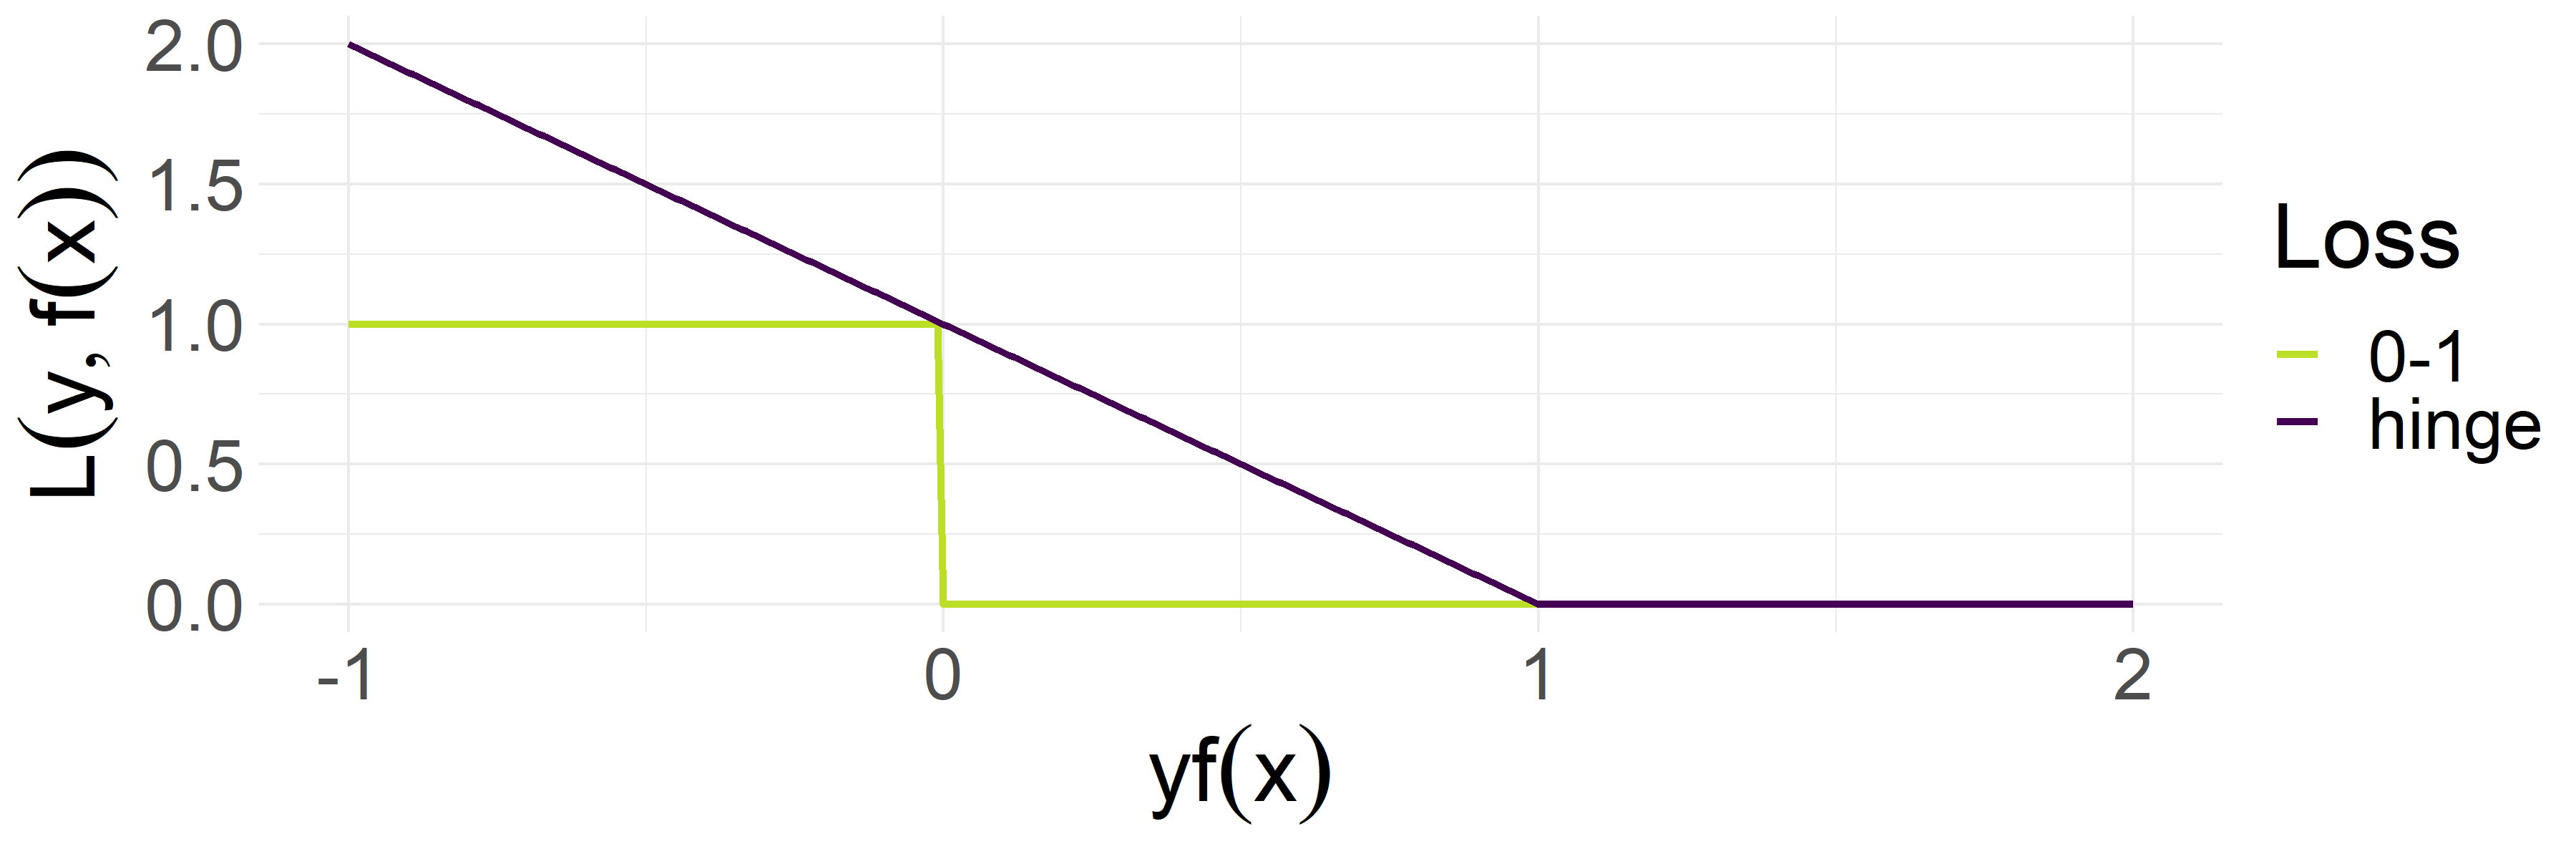
\includegraphics[height=\textwidth, keepaspectratio=true]{
  figure/plot_loss_hinge.png}
  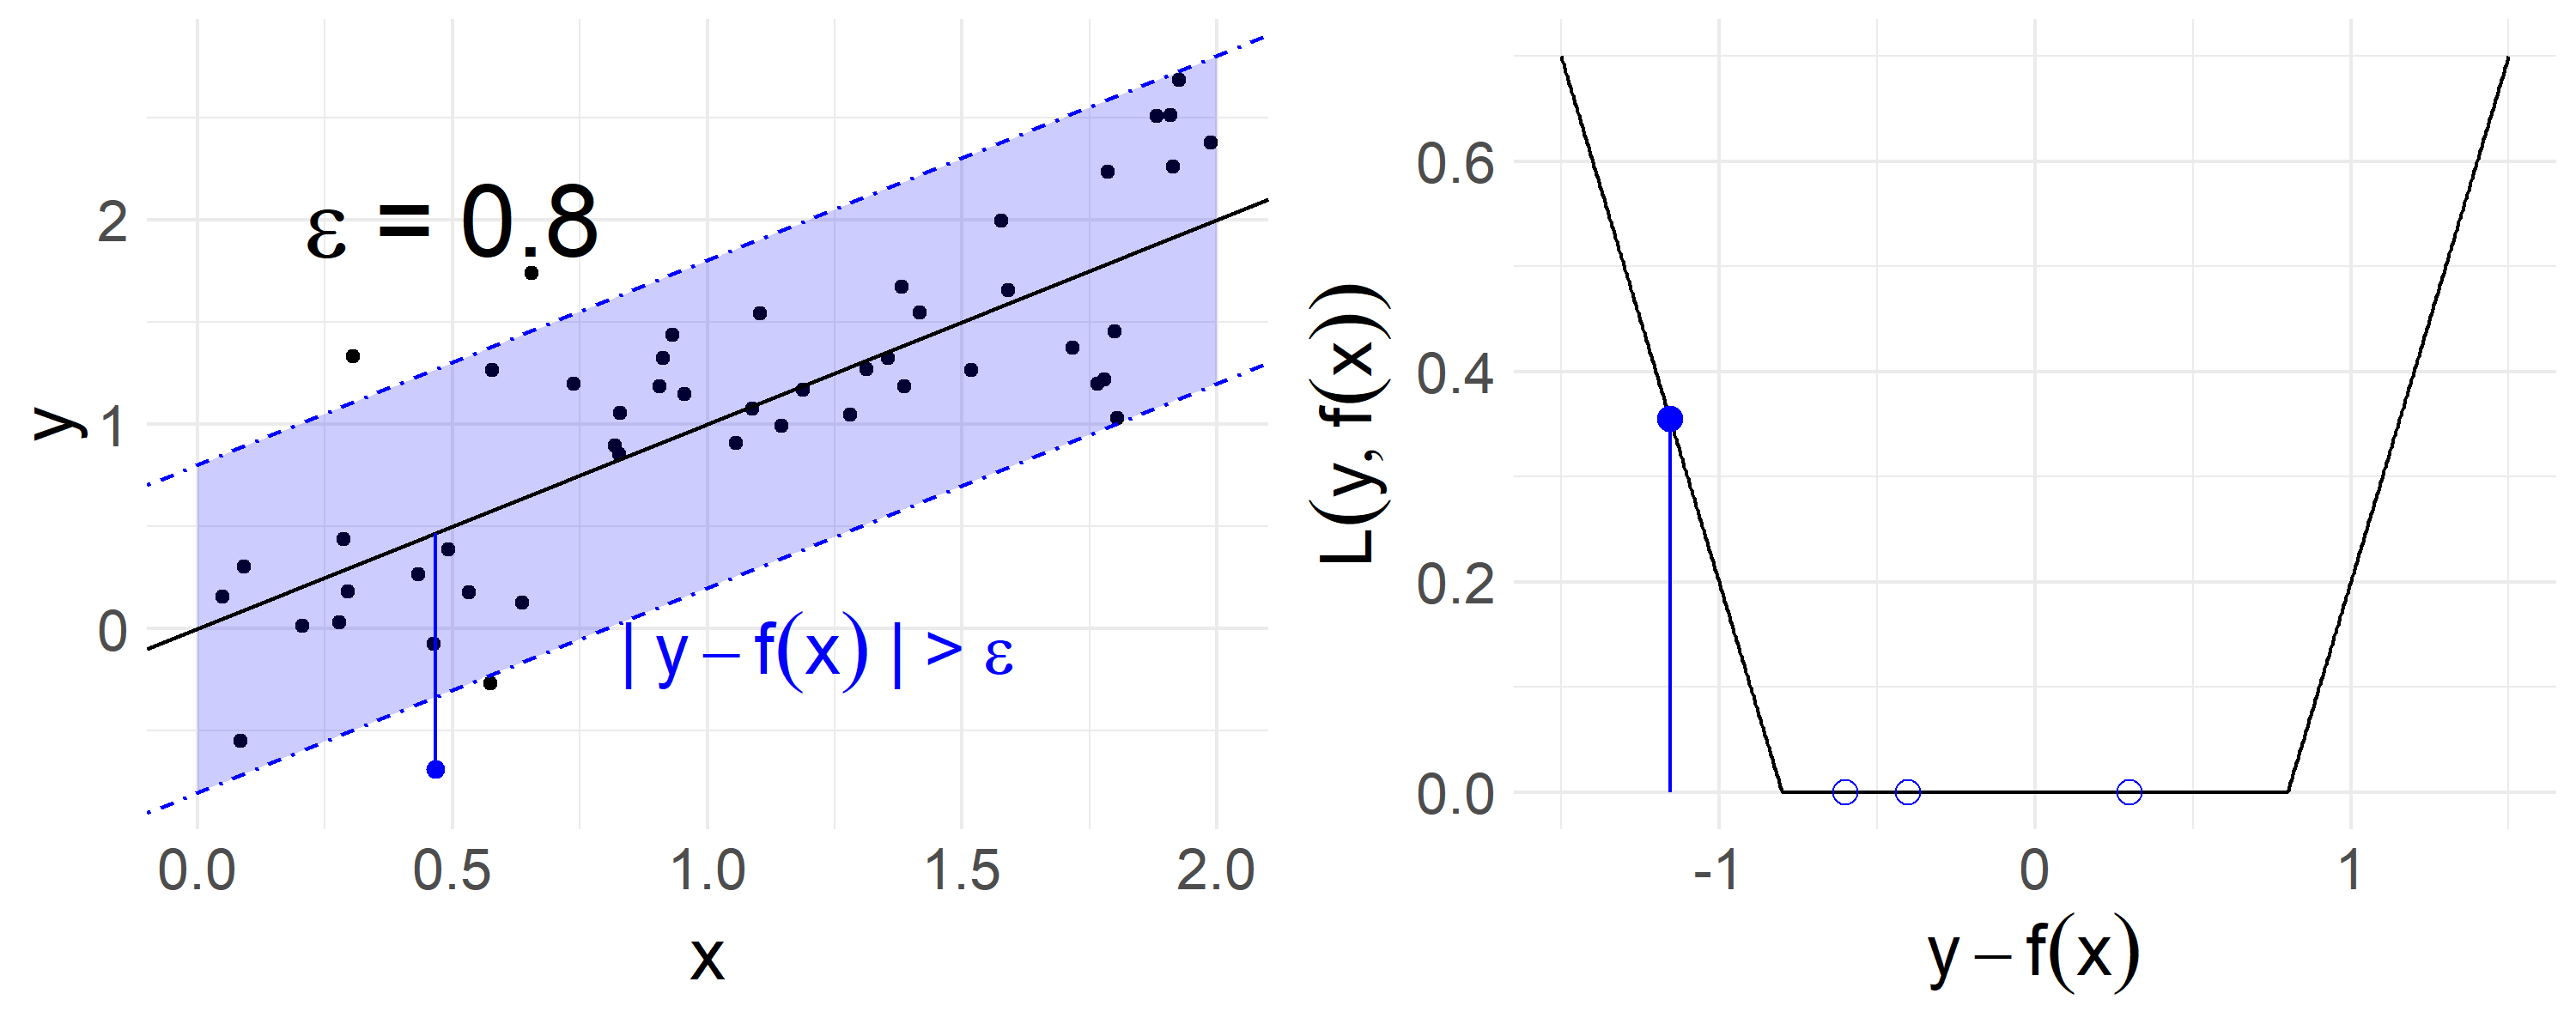
\includegraphics[height=\textwidth, keepaspectratio=true]{
  figure/loss_eps_insensitive.png}

\end{column}
\end{columns}

\medskip

\highlight{Dual problem} ~~ %lecture_cim2\2020\08-linear-svm\slides-3-soft-margin-svm.Rnw
%\textcolor{blue}{Motivation: \dots}
SVMs as a constraint optimization (primal) problem (maximize margin s.t. constraints on obs. to limit margin violations) can be formulated as a Lagrangian dual problem with Lagrange multipliers $\alpha_i \geq 0$: % by integrating the constraints to the objective using 
\begin{eqnarray*}
    & \max\limits_{\alphav \in \R^n} & \dualobj \\
    & \text{s.t. } & 0 \le \alpha_i \le C ~~ \forall i \in \nset \text{ and } \sum_{i=1}^n \alpha_i \yi = 0
\end{eqnarray*}

\framebreak

\highlight{Optimization}

\begin{itemize}
  \item Typically, tackling \textbf{dual} problem (though feasible 
  in corresponding primal) via \textbf{quadratic programming}
  \item Popular: \textbf{sequential minimal optimization} $\Rightarrow$ 
  iterative algorithm based on breaking down objective into bivariate quadratic 
  problems with analytical solutions
\end{itemize}
\medskip

\highlight{Hyperparameters} ~~ Cost parameter \textbf{$C$} to control maximization of the margin vs. minimizing margin violations

\hfill
\begin{columns}
    \begin{column}{0.5\textwidth}
    \centering
        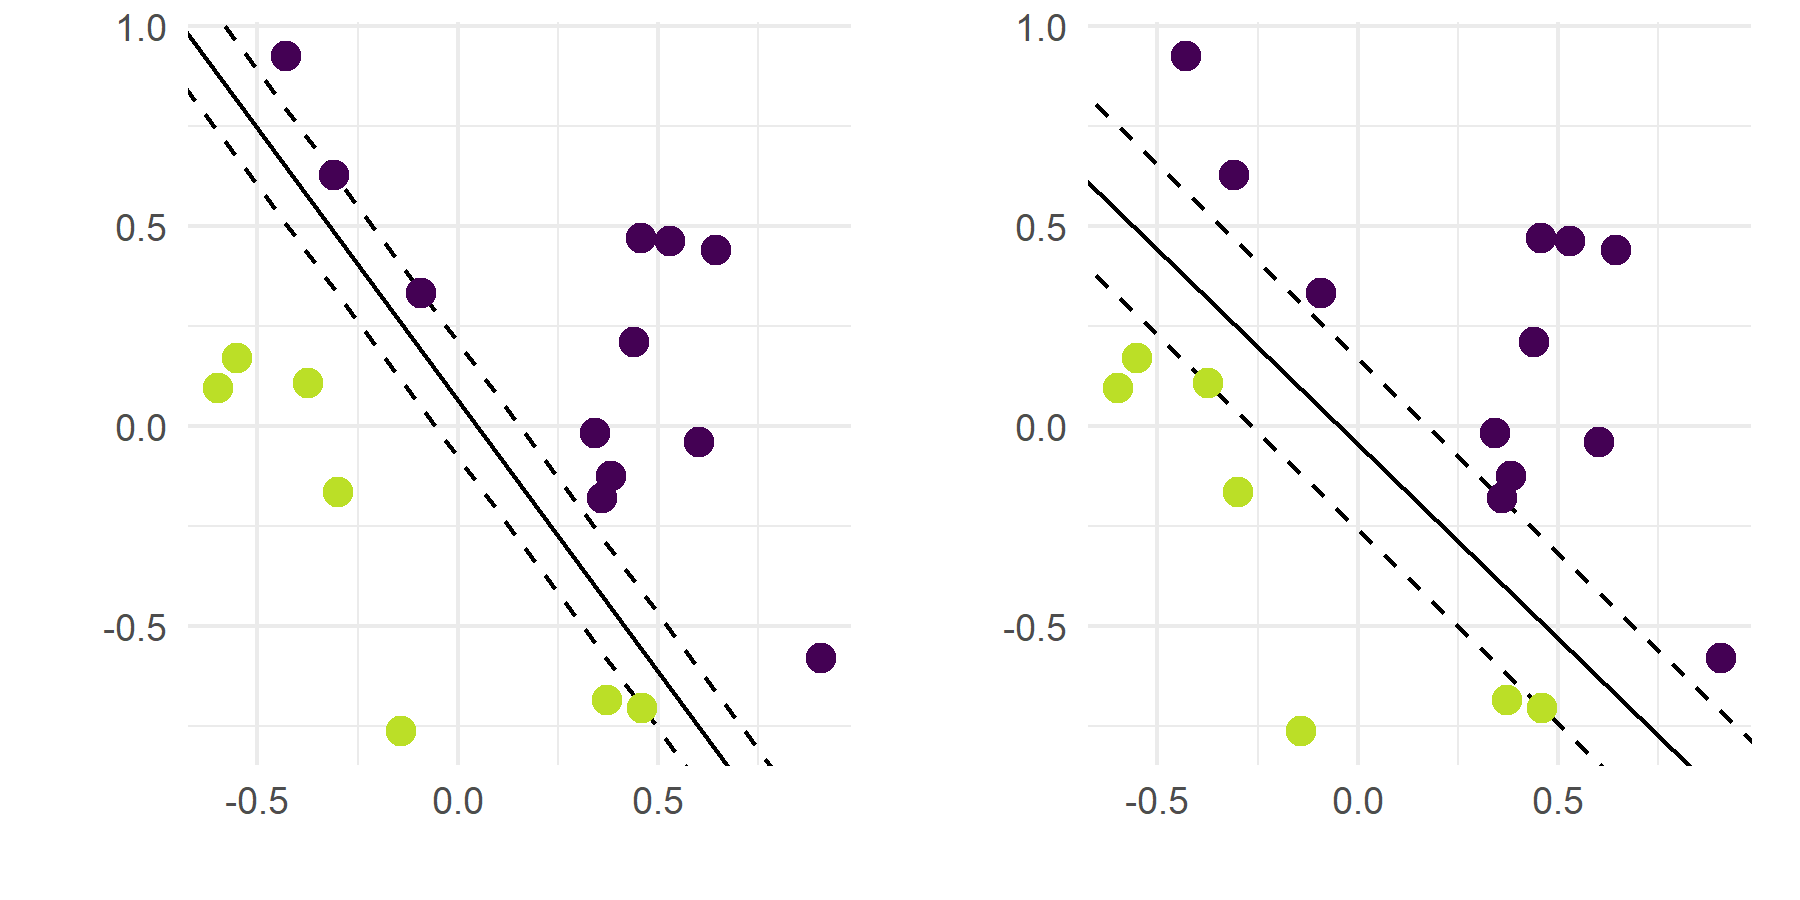
\includegraphics[width=\textwidth]{
  figure/linear_classif_2.png}  \\
  \tiny{Hard-margin SVM: margin is maximized by boundary on the right}
    \end{column}
    \begin{column}{0.5\textwidth}
    \centering
  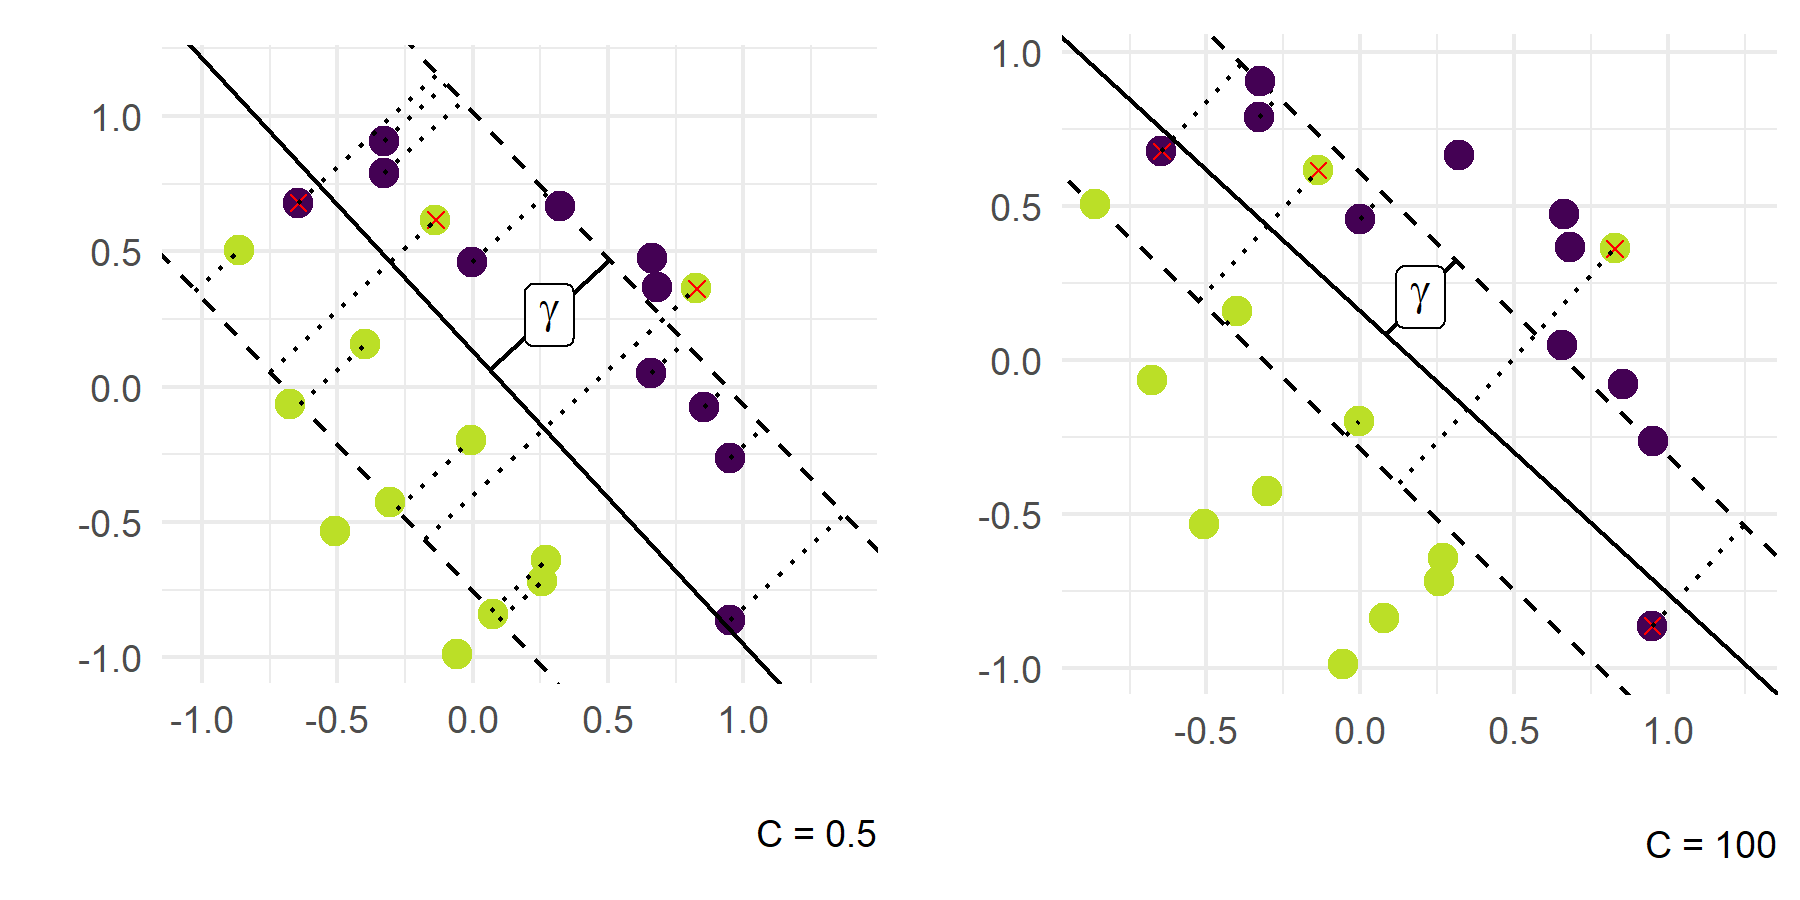
\includegraphics[width=\textwidth]{
  figure/margin_violations.png}  \\
  \tiny{Soft-margin SVM: large margin and few margin violations on the right (best trade-off)}
    \end{column}
\end{columns}

  \normalsize

\end{vbframe}


% ------------------------------------------------------------------------------

\begin{frame}{Linear SVM -- Practical hints}

\footnotesize

\highlight{Preprocessing} ~~
Features should be scaled before applying SVMs (applies generally to regularized models)

\medskip

\begin{columns}[T, totalwidth=\textwidth]
\begin{column}{0.52\textwidth}
    
\highlight{Tuning}

\begin{itemize}
  \item Tuning of cost parameter $C$ advisable\\
  $\Rightarrow$ strong influence 
  on resulting hyperplane
  \item $C$ it is often tuned on a log-scale grid for optimal and space-filling search space
\end{itemize}

\end{column}
    \begin{column}{0.45\textwidth}
        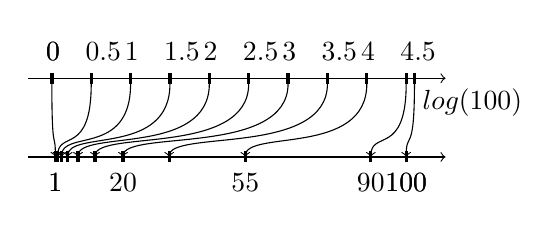
\begin{tikzpicture}[scale=1]
    \draw [->](-0.3,0)-- (5,0) coordinate;
    \draw [->](-0.3,-1)-- (5,-1) coordinate;
    \foreach \x/\xtext/\xxtext in {0/0/1,0.5/0.5/,1/1/,1.5/1.5/,2/2/,2.5/2.5/,3/3/20,3.5/3.5/,4/4/55,4.5/4.5/90,4.60517//100} {
      \draw [very thick] (\x,-2pt) -- ++(0, 4pt) node[xshift = -6pt, yshift=-3pt,anchor=south west,baseline]{\strut$\xtext$};
      \draw [very thick] ({exp(\x)*4.5/100},-1cm+2pt) -- ++(0,-4pt) node[anchor=north]{$\xxtext$};
      \draw [->] (\x,-2pt) .. controls (\x,-1) and ({exp(\x)*4.5/100},-0.65) .. ({exp(\x)*4.5/100},-1cm);
    }
    \draw [very thick] (0,-2pt) -- ++(0, 4pt) node[xshift = -6pt, yshift=-3pt,anchor=south west,baseline]{\strut$0$};
    \draw[very thick] (4.60517,2pt) -- ++(0,-4pt) node[xshift = -1pt, yshift=3pt,anchor=north west,baseline]{\strut$log(100)$};
    \draw [very thick] (4.5/100,-1cm+2pt) -- ++(0,-4pt) node[anchor=north]{$1$};
    \draw [very thick] (4.5,-1cm+2pt) -- ++(0,-4pt) node[anchor=north]{$100$};
  \end{tikzpicture}
    \end{column}
\end{columns}
\medskip

\highlight{Implementation} 
\begin{itemize}
  \item \textbf{R:} \texttt{mlr3} learners \texttt{LearnerClassifSVM} /
  \texttt{LearnerRegrSVM}, calling \texttt{e1071::svm()} with linear kernel (\texttt{libSVM} interface).
  Further implementations in \texttt{mlr3extralearners} based on
  \begin{itemize}
      \item \texttt{kernlab::ksvm()} allowing custom kernels
      \item \texttt{LiblineaR::LiblineaR()} for a fast implementation with linear kernel
  \end{itemize}
  \item \textbf{Python:} \texttt{sklearn.svm.SVC} from package 
  \texttt{scikit-learn} / package \texttt{libSVM}
\end{itemize}

\end{frame}

% % ------------------------------------------------------------------------------

% \begin{frame}{Linear SVM -- Pro's \& Con's}

% \begin{columns}[onlytextwidth]
%   \begin{column}{0.5\textwidth}
%     \highlight{Advantages}
%     \footnotesize
%     \begin{itemize}
%       % \positem High \textbf{accuracy}
%       \positem Often \textbf{sparse} solution (w.r.t. observations)
%       \positem Robust against overfitting (\textbf{regularized}); especially in 
%       high-dimensional space
%       \positem \textbf{Stable} solutions (w.r.t. changes in train data)\\
%       $\rightarrow$ Non-SV do not affect decision boundary
%       \positem Convex optimization problem \\
%       $\rightarrow$ local minimum $\hat{=}$ global minimum
%       %\positem \textbf{memory efficient} (only use non-SVs)
%     \end{itemize}
%   \end{column}

%   \begin{column}{0.5\textwidth}
%     \highlight{Disadvantages}
%     \footnotesize
%     \begin{itemize}
%       \negitem \textbf{Long} training times $\rightarrow O(n^2 p + n^3)$
%       %\negitem \textbf{Limited scalability} to larger data sets 
%       %\textcolor{blue}{\textbf{??}}
%       \negitem Confined to \textbf{linear model}
%       \negitem Restricted to \textbf{continuous features}
%       \negitem Optimization can also fail or get stuck
%       % \negitem Poor \textbf{interpretability}
%       %\negitem No handling of \textbf{missing} data
%     \end{itemize}
%   \end{column}
% \end{columns}

% \vfill

% \small

% \conclbox{Very accurate solution for high-dimensional data that is linearly 
% separable}

% \end{frame}